\section{Il commence a faire chaud}

Date: 18/02/2008

\begin{multicols}{2}

Aujourd'hui, je vais vous livrer un petit secret : nos 3 phrases préférées du moment :
- "Dure la vie hein!", à prendre évidemment au second degré. On dort dans des hôtels sympa, on mange dans des restos très bons avec des vues exceptionnelles, le petit vent chaud du soir est très agréable, les palaces sont plus beaux les uns que les autres...
- "Ca fait combien de temps qu'on n'a pas vu un nuage?" La réponse commence à s'approcher gentiment de "deux semaines". Et oui, que du grand ciel bleu à l'horizon, du lever au coucher du soleil (qui sont toujours rouges, bleus, verts et violets on tient à préciser).
-"Ils sont fous, vraiment, complètement fous je te dis". Les Indiens bien sûre, on n'a pas idée de construire autant de merveilles au kilomètre carré. Les yeux grands ouverts on arrive toujours pas à tout capter ce qui se présente devant nous. Toutes les sculptures, tous les détails, le zèle des batisseurs... c'est incroyable.

Et au dela de ces impressions générales qui se confirment de jour en jour, nous continuons notre périple. Nous avons quitté notre hôtel ce matin à 5h, puis 3 grosses heures de bus pour arriver à Ranakpur. Là se trouve un des plus importants temples Jain de l'Inde, plus trois autres plus petits. Le gros comprends 29 pièces, et pas moins de 1444 colonnes de marbres sculptées (oui ils sont fous, on vous avait bien dit hein!). Les temples sont encastrés entre les montagnes, toutes recouvertes de verdure. On a même le plaisir de nourir les singes qui viennent calmement prendre des morceaux de gâteaux qu'on leur tend. Encore une halte fort agréable. Le soir, 4h30 de bus pour rejoindre Jodhpur où nous sommes actuellement. Ca semble promettre des moments sympa, surtout que nous allons y rester 5 ou 6 jours, jusqu'au moment de rentrer à Delhi pour faire des achats et prendre l'avion de retour. Et oui, on va être obligés de rentrer au bout d'un moment! En tout cas, on ne pense pas encore vraiment à ça et on profite à fond de chaque petit moment, de tout ce qui peut nous émerveiller : un oiseau vert et orange, des femmes rentrant des champs portant des fagots sur leur tête, des maisons de toutes les couleurs, les femmes qui lavent le linge sur les ghats... Nous passons tellement de moments intenses et indescriptibles! Le City Palace d'Udaipur qui s'illumine le soir, un spectacle de danse rajasthanie , la rencontre d'Indiens, mais aussi d'autres touristes, Européens, Américains ou encore Francais. On comprend de mieux en mieux l'anglais des Indiens et on relance les conversations. Nous croisons beaucoup de gens, mais brièvement. Nous nous fondons aussi de mieux en mieux dans le paysage, portant des habits plus "cool" et connaissant maintenant les combines des marchands. On ne prévoit plus ce qu'on fait, mais seulement on vit le moment à fond. Car l'Inde est un pays qui ne se raconte pas, mais qui se vit. Les photos sont peut-être jolies et les textes vous plaisent, mais tout ça n'est rien du tout par rapport à la réalité que nous vivons avec un grand plaisir chaque jour, chaque minute. Souvent les mots manquent pour exprimer ce que l'on ressent. On se contente alors d'un silence, d'un regard entre nous et d'un large sourire tout au fond du coeur. On ne réinventera pas les mots, nul besoin, car on sait très bien au fond de nous l'effet que ça produit, la trace que ça laissera, et c'est bien le principal.

\hspace*{-0.65cm}
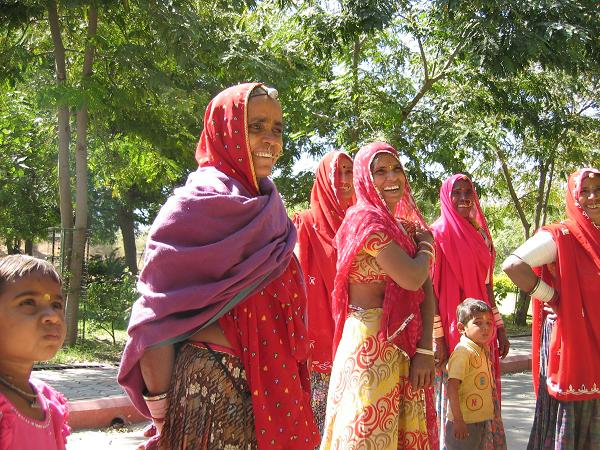
\includegraphics[width=4.8cm]{articles/Il-commence-a-faire-chaud/sari.jpg}
Des femmes en sari coloré

\hspace*{-0.65cm}
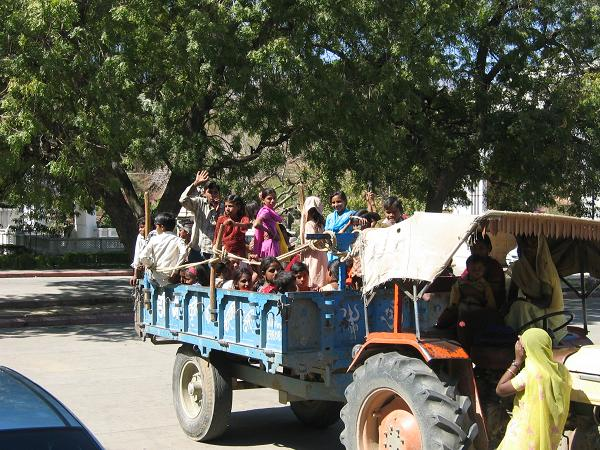
\includegraphics[width=4.8cm]{articles/Il-commence-a-faire-chaud/scolaire.jpg}
Un groupe d'enfants en sortie scolaire.

\hspace*{-0.65cm}
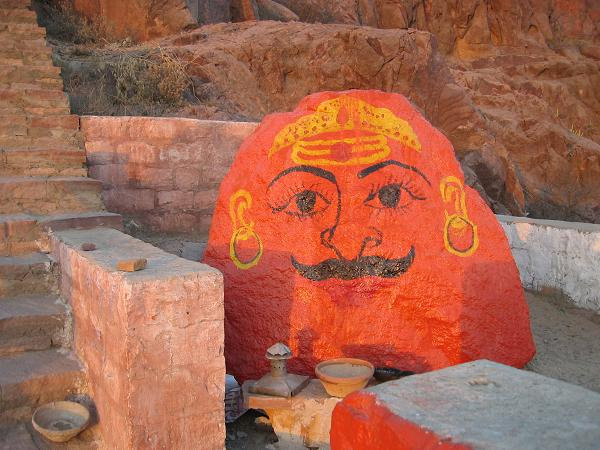
\includegraphics[width=4.8cm]{articles/Il-commence-a-faire-chaud/bonhommerouge.jpg}
Une icône peinte sur un rocher.

\hspace*{-0.65cm}
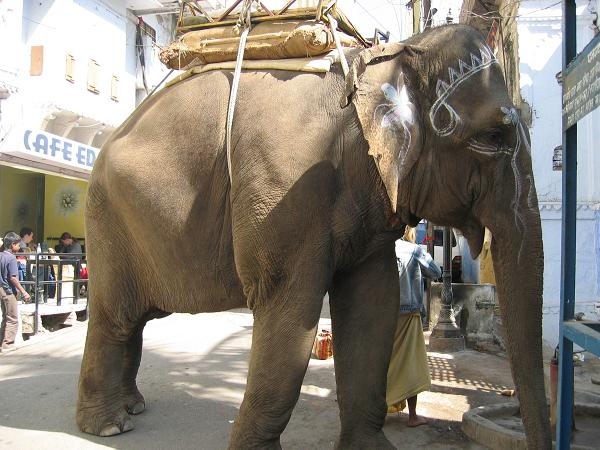
\includegraphics[width=4.8cm]{articles/Il-commence-a-faire-chaud/elephant.jpg}
Un éléphant dans une rue d'Udaipur.

\hspace*{-0.65cm}
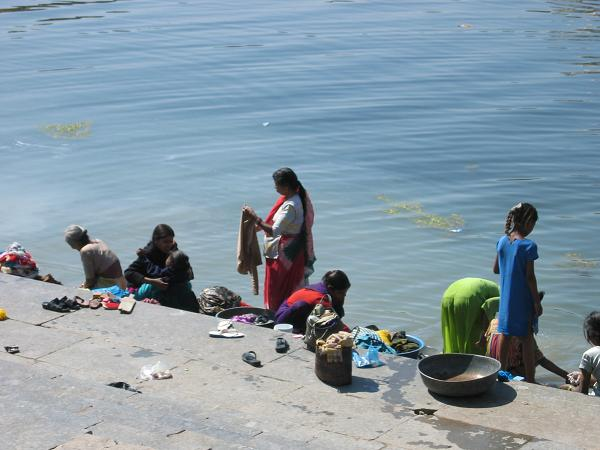
\includegraphics[width=4.8cm]{articles/Il-commence-a-faire-chaud/linge.jpg}
Des femmes lavant le linge sur les gaths.

\hspace*{-0.65cm}
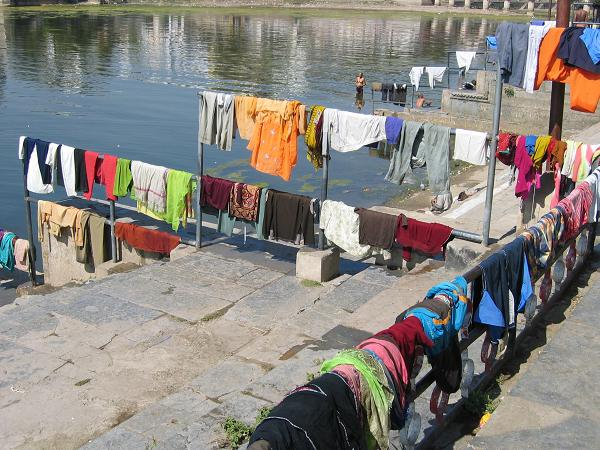
\includegraphics[width=4.8cm]{articles/Il-commence-a-faire-chaud/seche.jpg}
Le linge qui sèche.

\hspace*{-0.65cm}
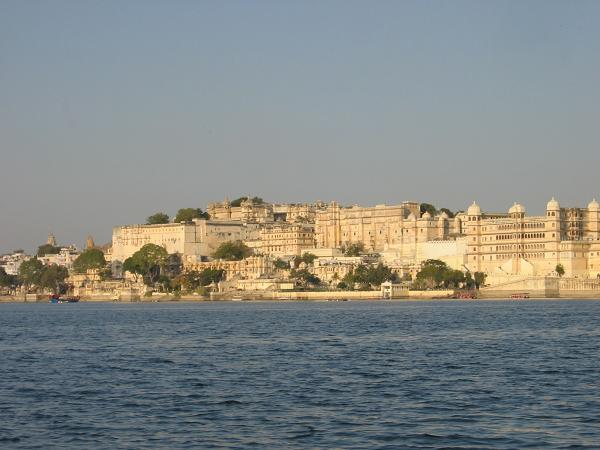
\includegraphics[width=4.8cm]{articles/Il-commence-a-faire-chaud/palacelac.jpg}
Le City Palace d'Udaipur vu depuis le lac.

\hspace*{-0.65cm}
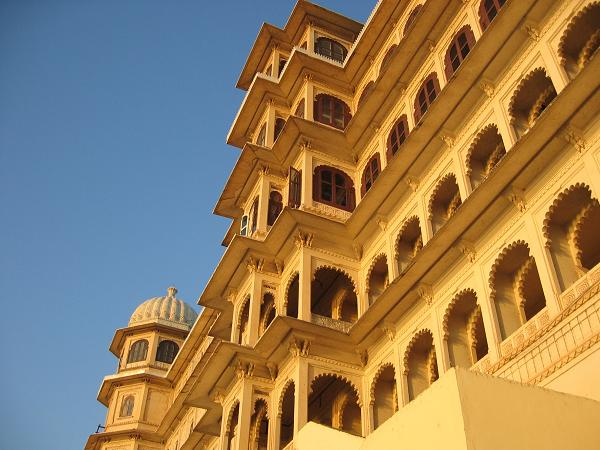
\includegraphics[width=4.8cm]{articles/Il-commence-a-faire-chaud/citylac2.jpg}
Une autre vue du City Palace.

\hspace*{-0.65cm}
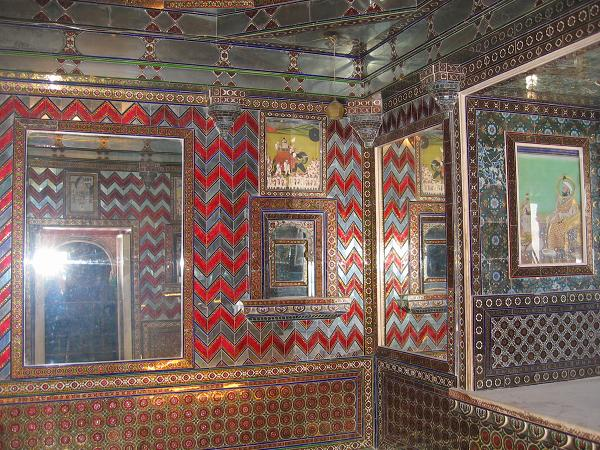
\includegraphics[width=4.8cm]{articles/Il-commence-a-faire-chaud/citysalle.jpg}
Une salle du City Palace.

\hspace*{-0.65cm}
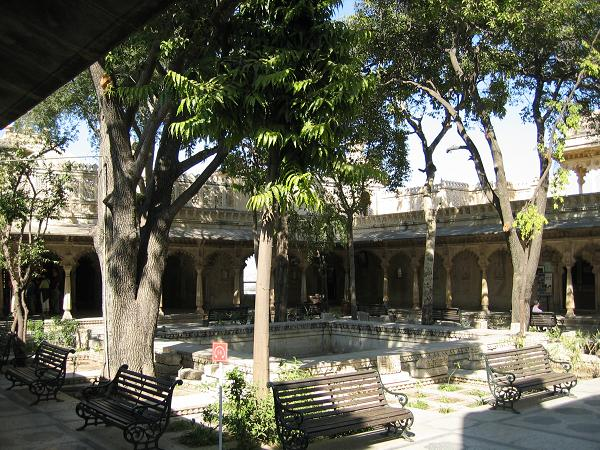
\includegraphics[width=4.8cm]{articles/Il-commence-a-faire-chaud/citycours.jpg}
Une cour intérieure.

\hspace*{-0.65cm}
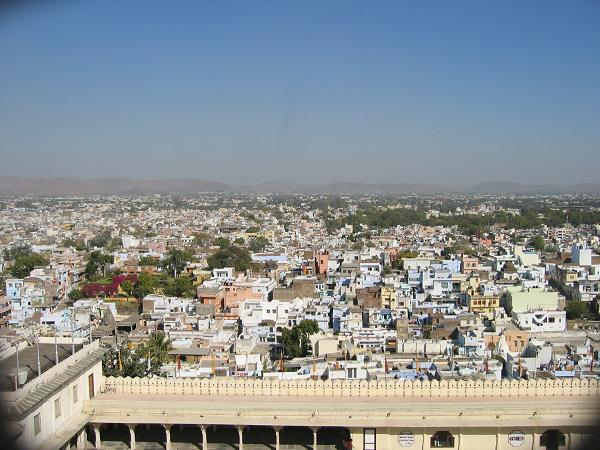
\includegraphics[width=4.8cm]{articles/Il-commence-a-faire-chaud/udaipur.jpg}
La ville d'Udaipur.

\hspace*{-0.65cm}
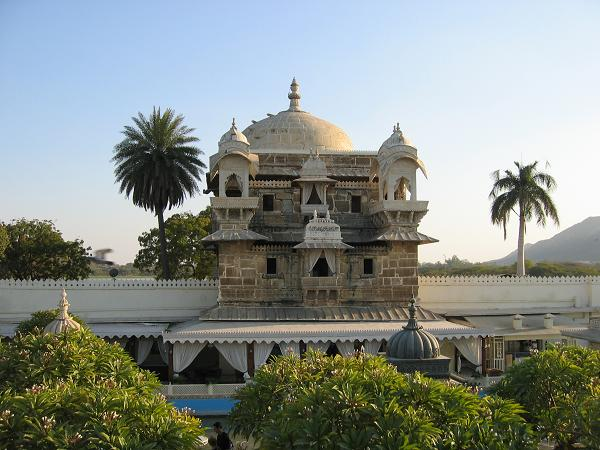
\includegraphics[width=4.8cm]{articles/Il-commence-a-faire-chaud/picchola.jpg}
Une belle vue depuis une île du lac Pichola.

\hspace*{-0.65cm}
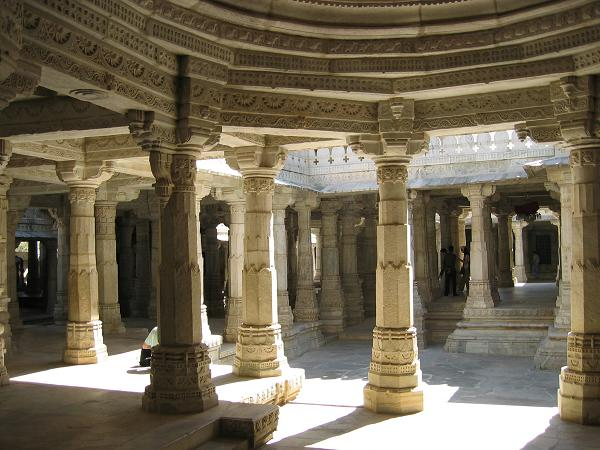
\includegraphics[width=4.8cm]{articles/Il-commence-a-faire-chaud/ranak.jpg}
Un immense temple Jain de Ranakpur.

\hspace*{-0.65cm}
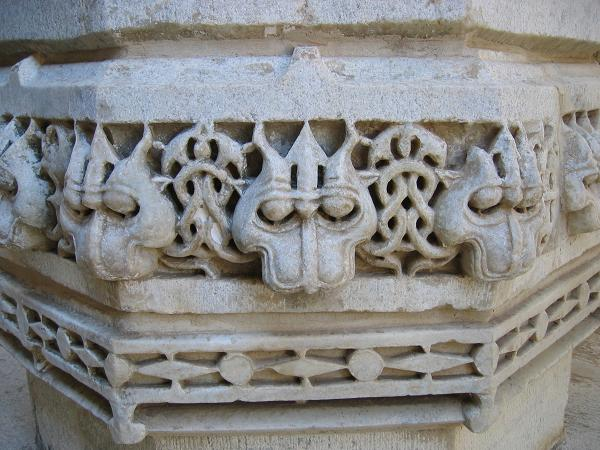
\includegraphics[width=4.8cm]{articles/Il-commence-a-faire-chaud/ranak2.jpg}
Le détail d'un temple.

\hspace*{-0.65cm}
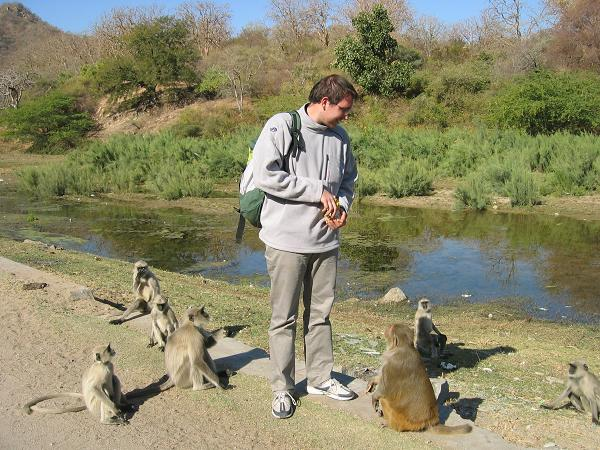
\includegraphics[width=4.8cm]{articles/Il-commence-a-faire-chaud/ranak3.jpg}
Etienne nourissant les singes.

\hspace*{-0.65cm}
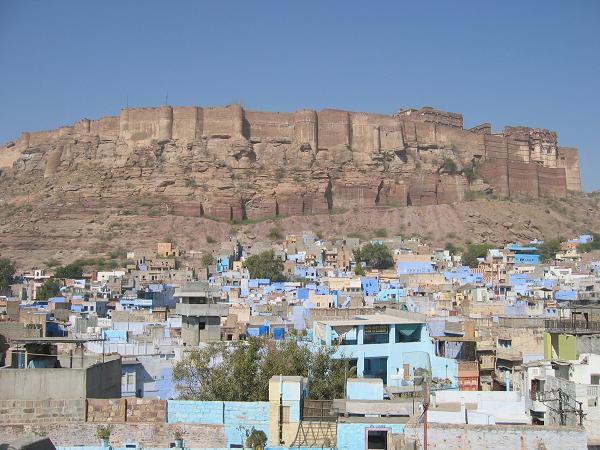
\includegraphics[width=4.8cm]{articles/Il-commence-a-faire-chaud/ranak4.jpg}
La vue depuis la terrasse de notre guest house de Jodhpur.

Allez, parce que vous êtes sages, vous avez le droit à une video bonus.

\end{multicols}

\bigskip
\textbf{\textsc{Commentaires}}

\medskip
Titou a écrit le 18 fév. 2008 :
\begin{displayquote}
Ra vous nouys faites rever meme sans les images. Je comprend ce que vous ressentez car je l'ai ressenti ici aussi meme si l'univers est completement different. C'est toujours tres dur de transmettre ce que l'on ressent et que l'on voit parfois tellement c'est beau. Ce qui prouve que notre monde regorge de choses magnifiques dont on ne soupsconne parfois pas l'existence\dots Profitez en toujours a fond, faites de ce sejour un souvenir memorable et on se revoit dans peu de temps. Faites gaffe a vous et a plus. Biz.
\end{displayquote}

\medskip
Lydie a écrit le 19 fév. 2008 :
\begin{displayquote}
Ahlala, vos paroles sont encore plus belles que les images. On se plonge avec "extase" à travers vos écrits !!!
Profitez-bien de vos derniers jours !!! Et j'attends de tes nouvelles ma poulette. Bisous.
\end{displayquote}

\medskip
Zan a écrit le 19 fév. 2008 :
\begin{displayquote}
Hébé, ça dépayse de la Franche-Comté\dots
Vous devez vraiment en avoir plein les yeux et les oreilles tous les jours (et ptet plein le c*l aussi des singes :D)!
Continuez de nous faire rêver avec ces photos, elles sont vraiment magnifiques!
@ bientôt!
\end{displayquote}

\medskip
Peggy a écrit le 20 fév. 2008 :
\begin{displayquote}
Etienne qui essaie d'apprendre aux singes les règles de bonnes conduites\dots j'adore!
\end{displayquote}

\medskip
Poun's a écrit le 20 fév. 2008 :
\begin{displayquote}
Salut vous deux, Bon, si vous continuez, on va affréter un avion pour vous rejoindre,,,,
La météo, toujours pas de nuages? On a l'impression qu'il ne fait pas toujours très chaud là-bas, Vous n'avz pas froid?
Continuez les photos, même si elles ne passent pas toutes, et surtout mettez-en plein votre tête pour nous raconter tout ça,
Félicitations au nouveau tonton, et surtout à la maman et au papa,
Ca tombe bien, je travaille à Besançon Vendredi, on va fêter ça!
A bientôt,
\end{displayquote}

\medskip
Tatid a écrit le 21 fév. 2008 :
\begin{displayquote}
J'ai toujours pas le net à l'appart, mais vu que j'ai pas grand chose à faire en stage, j'en profite pour ratrapper ma lecture de blogs (j'ai lu l'intégral de "Fab aux USA" en 2 jours ^^) !
Vos photos sont vraiment superbes, c'est dingue le changement de culture par rapport à la notre, ça doit être vraiment enrichissant un voyage comme ça, puisqu'on est plus du tout dans la culture occidentale quoi ! Les monuments sont aussi impressionnants de beauté ! En tous cas, vous n'avez pas l'air triste (c'est le moins qu'on puisse dire !) et vous avez l'air d'en avoir profité au maximum, c'est génial !
Dis Dud, tu t'es fait des potes singes ? T'en ramène un nan ?! ^^
\end{displayquote}

\medskip
Etienne a écrit le 21 fév. 2008 :
\begin{displayquote}
Alors question meteo ca commence a chauffer. On a deja du avoir du 30 degres je pense. Merci bien pour les felicitation, je transmettrais avec grand plaisir a ma soeurette car elle ne doit plus trop avoir le temps de venir lire ce blog a mon avis\dots
Bernard, a vendredi ;-)
Tatid, on m'a meme propose de m'en vendre un a Agra, le mec rigolais devant ma tete de tourist a regarder le singe sur le toit de sa shop "You want it ? i give you for 100 Rs".
Continuez a nous ecrire comme ca, ca fait tres plaisir de voir que notre voyage est suivi. C est a chaque fois le suspense quand on va sur internet. A bientot.
\end{displayquote}

\medskip
Soeurette\dots a écrit le 21 fév. 2008 :
\begin{displayquote}
Comment ça j'ai ps le temps de vous lire\dots !!! je suis là\dots bon d'accord, je suis pas venu depuis un bon bout de temps, mais je ratrape mon retard ce soir pendant que Lucie dort\dots
Ce n'est pas l'endrois, mais j'en profits pour dire à tout ceux  qui me lirons que l'acouchement à été un peu dur, mais tout va bien maintenant. Ca fais du bien d'ètre chez sois\dots et Lucie à l'aire de se plaire chez elle\dots
Maintenant que j'ai parler de moi, j'espère que vous reviendrez de ce voyage plein de bons souvenir dans la tête\dots j'imagine que à peine rentré, vous allez avoir envie de repartir visiter le monde ?
Aller, continuez bien, à mardi prochain.
Bisou
Cécile la soeurette\dots
\end{displayquote}

\medskip
Gerien a écrit le 22 fév. 2008 :
\begin{displayquote}
Alors la grande question de la pause café de ce matin à l'alstom c'est :
Est ce que dud c'est fait bouffé la main par un singe (surtout le gros là à la fin) ?
Allez, bonne fin de voyage les gens ;o)
\end{displayquote}

\medskip
Etienne a écrit le 23 fév. 2008 :
\begin{displayquote}
Hehe\dots je voit que ca bosse dur dans les bureau d'Alstom\dots
Les singes etaient trop content qu'on leur donne a manger pour etre agressifs, en fait ils doivent avoir l'habitude car il y a beaucoup de passage la ou on etait. Mais par contre on en a deja vu flanquer la frousse a une touriste jusqu'a ce qu'elle lache la pomme qu'elle etait en train de manger, et ca c'est assez impressionnant a voir, on doit rapidement se dire qu'une pomme ne vaut pas une morsure de singe.
\end{displayquote}

\medskip
Poun's a écrit le 23 fév. 2008 :
\begin{displayquote}
Salut à vous. N'oubliez pas de prendre des pommes, si ça peut vous sauver une main\dots
Pensez à ma commande : une vache sacrée, un singe, 1 l'd'eau du Gange et si vous avez un peu de place dans vos bagages, un éléphant me serait très utile.
A bientôt pour vos nouvelles aventures, j'espère que vous ne mourez pas de chaud.
\end{displayquote}

\medskip
Gerien a écrit le 24 fév. 2008 :
\begin{displayquote}
Moi, ce que je commanderais prendrais moins de place\dots
:)
\end{displayquote}

\vfill

